%!TEX root = nips2015.tex

\section{Deep Q Learning for solving Go}
In this section, we detail our initial motivation behind using the Deep Q Learning to solve Go. As detailed in the previous section, Go has been traditionally solved using Monte Carlo which searches through the complete state space of Go, however its time consuming considering the size of Go's state space. 
\\
A more elegant approach which is used by human experts is through finding shapes. Professional players analyse positions using a large vocabulary of shapes, such as joseki (corner patterns) and tesuji (tactical patterns). The most simple example is that of an atari which is shown in \textcolor{red}{Figure } to illustrate the idea. If we regard the game as an image, then a Convolution Neural Network can identify these patterns. This is probably the reason behind success of convolution neural network. However a CNN can only look through the next move and thus fares badly against a Monte Carlo which can evaluate multiple moves.
\\
\begin{figure}[h]
	\centering
	\subfloat[Example 1: The white stones are all in atari and can be captured if black plays the next move]{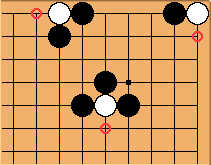
\includegraphics[width=0.47\textwidth]{atari_1}\label{fig:Gamma_0.7}}
	\hfill
	\subfloat[Example 2:The five black stones on the top right are in atari. The only liberty they have is the circled intersection.
	The group of two black stones on the lower left is also in atari. It may be captured by white (when white plays at a).]{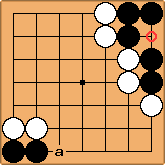
\includegraphics[width=0.43\textwidth]{atari_2}\label{fig:Karpathy}}
	\caption{Concept of Atari}
\end{figure}
\\
Our approach combines the benefit of visualizing shapes through CNN and looking ahead through Q Learning using a discount factor greater than 0. It is similar to the approach used by Facebook but it is more elegant as look ahead and shape recognition are combined in the same algorithm rather than being separate.